\documentclass{article}[12pt]
\usepackage{amsmath}
\usepackage{hyperref}
\usepackage{graphicx}
\graphicspath{ {./images/} }
\newcommand{\rot}[3]{#3#2#1}
\newcommand{\myskip}{\bigskip\noindent}

\title{Interpreting Neural Nets by Training to Reduce Nonlinearities}
\author{Elod Pal Csirmaz\\
\texttt{\rot{\rot{maz.}{csir}{ep}com}{@}{elod}}}

\date{\today}
\begin{document}

\maketitle

\begin{abstract}
Machine learning and neural networks are used more and more widely,
despite the fact that they mostly function as black boxes, and we
have little insight into how they reach decisions.
This makes it difficult to scrutinize and account for decisions made using these systems.

In this paper we present a simple solution that makes it possible to
extract rules from a neural network that employs Parametric Rectified Linear Units (PReLUs).
We introduce a force, applied in parallel to backpropagation, that
aims to reduce PReLUs into the identity function, which then causes
the neural network to collapse into a smaller system of linear functions and inequalities
suitable for review or use by human decision makers.

As this force reduces the capacity of neural networks, it is expected to help avoid overfitting as well.

\myskip
{\bf Keywords:} % (4-6)
machine learning,
neural networks,
rule extraction

\myskip
{\bf MSC classes:} % http://www.ams.org/mathscinet/msc/msc2010.html
62M45,  % Neural nets and related approaches
68T05   % Learning and adaptive systems

% \myskip
% {\bf ACM classes:} % http://www.acm.org/about/class/ccs98-html

\end{abstract}

\section{Introduction}

Machine learning solutions and, more specifically, neural networks are used
in more and more areas of our lives. At the same time, since it is difficult to 
grasp at any level how they function and so they can be seen as black boxes,
there is a reluctance in their adoption in the case of companies who need to
remain accountable for business and/or legal reasons. This fact also impacts
the trust the public places in such systems.

Because of this, providing tools that can help us understand how these
models arrive at a certain decision is an area of active research.
The tools range from visualization tools, tools that identify the
most significant input, tools that allow experimenting with the input data
to understand the relative importance the model attributes to different
signals, and, the focus of this paper, significantly reducing the complexity
of a neural network to the point where ``rules'' for decisions could be
extracted from it, which can then be reviewed or even used by human decision-makers.

One form these rules can take is a closed, relatively simple algebraic
expression (for example, a linear function) which has a behavior more
predictable for humans than the full function implemented by a neural
network involving parameters and nonlinear functions in the range of
millions.

In this paper we detail a method of reducing the complexity of a neural
network during its training, which then allows describing its output as a
simple system of linear functions limited to regions defined by linear
inequalities.
In particular,
we investigate feed-forward neural networks
where all nonlinearities are Parametric Rectified Linear Units (PReLUs)
defined as
\[ f(x) = \max(0, x) + a \min(0, x). \]
where $0\leq a\leq 1$.\cite{PR}

Let the input of the network be the vector (or tensor, which we flatten) $I=(i_1, i_2, \ldots, i_n)$
and the output be the vector (or tensor) $O=(o_1, o_2, \ldots, o_m)$.

\section{The Neural Network as a Combination of Linear Functions}

It is easy to see that the output $O$ of such a network can be expressed
as a set of linear combinations of $i_x$, each restricted to a particular region of input values
by a set of linear inequalities on $i_x$ (the conditions).

Intuitively, this is true because the output is a linear function of the input
as long as (that is, inside regions of the possible input vectors in which) none of the inputs of PReLUs
cross from negative to positive or \emph{vice versa}; and because the borders of these regions
are linear as well.

More formally, we can show that this statement is true by constructing a suitable
system of linear combinations and inequalities for any given neural network.
For all PReLUs in the network, let us decide whether their inputs are negative, or nonnegative.
If the number of PReLUs is $\delta$, this means $2^\delta$ possible scenarios.
In each scenario, the neural network becomes completely linear, with the output being a linear function of the input,
and, in fact, with all partial results inside the network being linear functions of the input as well.
This entails that the inputs of PReLUs are also linear functions of the input $I$, yielding
the $\delta$ linear inequalities (the conditions) that mark out the region of the input space where this scenario applies.

Naturally, this system of $2^\delta$ linear combinations yielding the output, each controlled by $\delta$
conditions is likely to be redundant, as the conditions may not be independent,
or may be contradictory, in which case some of the $2^\delta$ regions of the input space will be empty.
But this system will be an accurate description of the output of the neural network nevertheless.

\myskip
While a linear function may seem easy to interpret and to predict for us humans, clearly $2^\delta$
functions will not be so if $\delta$ is in the range of thousands or millions as in most modern neural networks.
We therefore need to construct an approximation of the output of our neural network which is linear in much
larger regions of the input space, and has far less different regions as well.
This is equivalent to trying to find another neural network that approximates our network well,
but contains a small number of PReLUs only.

\section{Reducing PReLUs into Linearities}

We achieve this by continuing training the original neural network while applying a force on each of
its PReLUs that moves its parameter $a$ towards 1.

Note that if $a=1$, then the PReLU degenerates into the identity function $f(x)=x$, and ceases to be a nonlinearity.
In a sense, it disappears, and the neural network ``collapses'' around it, inasmuch as the linear mapping
that precedes the degenerate PReLU and the one after it can now be combined into a single linear map.

This force therefore finds a balance between approximating the training data
and reducing the number of PReLUs, thereby yielding a neural network that is feasible to express
as a set of linear functions and inequalities for human consumption.
By removing nonlinearities, this force also reduces the capacity of the neural network,
and therefore we expect that it can also be helpful to avoid overfitting.

We chose a
force that is a static and is applied after each backpropagation step, and moves the parameter by an adjustment rate
$\eta_p$ but never above 1:
\[ a_{t+1} = \max\left(0,\;\min\big(1,\;a_t + \eta_p\,\mathrm{sgn}(1-a_t)\,\big)\right) \]

In our research we considered any PReLU fully linear if
\[ a > 0.9995 \]

We also made $\eta_p$ dependent on the current error exhibited by the network,
to allow the network initially to train without interference, and then
pull the PReLU parameters to 1 more and more aggressively. We chose
\[ \eta_p = \eta_0\,0.01\,\max\big(0,\; -\log_{10}(err)-2\big) \]
where $\eta_0=0.01$ is the learning rate for the whole model, and $err$ is the training error.
This means that $\eta_p$ will start becoming non-zero when the training error
falls below 0.01, and can grow indefinitely as the training error falls
(although the $a$ parameters are clipped anyway).

\section{Example}

Sample code demonstrating the above is available at
\url{https://github.com/csirmaz/trained-linearization}.
The code implements training a small neural net with the force on PReLU parameters,
and contains logic to extract a system of linear inequalities and combinations
from the weights and other parameters of the model.

The neural network itself
has 4 input nodes, 3 output nodes, and
4 hidden layers in between with 5 nodes on each.
These layers are linked by trainable fully-connected layers
with PReLU activation following them, except for the last fully connected layer,
which simply provides the output.

The network is expected to learn the following relationships:
\begin{align}
\mathrm{out}_1 &= \mathrm{in}_1 \;\mathrm{xor}\; \mathrm{in}_2 \\
\mathrm{out}_2 &= \mathrm{in}_3 \;\mathrm{xor}\; \mathrm{in}_4 \\
\mathrm{out}_3 &= \mathrm{in}_1 \cdot \mathrm{in}_2
\end{align}
where all the inputs and outputs are 0 or 1 with some extra noise added to the inputs.
We generate the training data according to the expressions above, for all $2^4$ possible combinations of 0 and 1 for the input.
New noise is generated for each batch of training data.

\begin{figure}[ht]
\centering
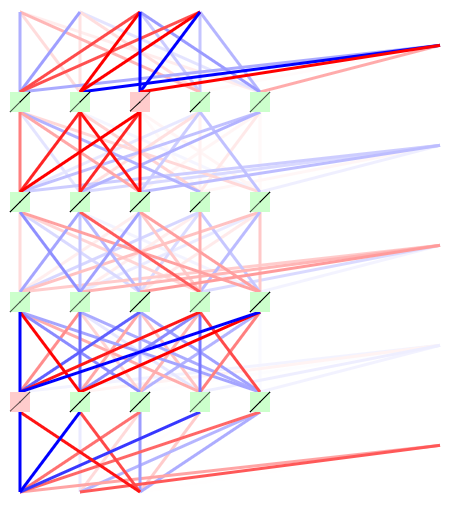
\includegraphics[height=10cm]{example}
\caption{A trained network with 4 input nodes (top) and 3 output nodes (bottom). Red lines denote positive, blue lines negative weights.
Lines leading from the right denote bias values. Green boxes mark PReLUs that are considered linear, while red ones mark nonlinear PReLUs.}
\label{fig}
\end{figure}

Figure \ref{fig} visualizes a trained model. Two nonlinearities are enough to solve this problem, and indeed the training
settled on a solution where only two PReLUs were nonlinear.

Although in the visualization the relationships between the inputs and the outputs are far from clear,
once the rest of the PReLUs are considered linear, all the weights collapse into very simple expressions.
See figure \ref{output} for the output of the code listing these expressions for the $2^2$ cases arising from the
two nonlinear PReLUs.
These correspond completely to the relationships in the training data.

\begin{figure}[ht]
\begin{verbatim}
IF +0.00*in1 +0.00*in2 -1.00*in3 -1.00*in4 +1.00 < 0
   (PReLU #3 on level 1 is neg. ln(1-weight)=-2.58)  
IF +1.00*in1 +1.00*in2 -0.00*in3 -0.00*in4 -1.00 < 0
   (PReLU #1 on level 4 is neg. ln(1-weight)=-2.60)  
THEN    
  out1 = +1.01*in1 +1.01*in2 -0.00*in3 -0.00*in4 +0.00  
  out2 = -0.00*in1 -0.00*in2 -1.03*in3 -1.03*in4 +2.04  
  out3 = -0.00*in1 -0.00*in2 +0.00*in3 +0.00*in4 -0.00  
        
IF +0.00*in1 +0.00*in2 -1.00*in3 -1.00*in4 +1.00 < 0
   (PReLU #3 on level 1 is neg. ln(1-weight)=-2.58)  
IF +1.00*in1 +1.00*in2 -0.00*in3 -0.00*in4 -1.00 > 0
   (PReLU #1 on level 4 is pos. ln(1-weight)=-2.60)  
THEN    
  out1 = -1.01*in1 -1.01*in2 +0.00*in3 +0.00*in4 +2.02  
  out2 = -0.00*in1 -0.00*in2 -1.03*in3 -1.03*in4 +2.04  
  out3 = +1.00*in1 +1.00*in2 +0.00*in3 +0.00*in4 -1.01  
        
IF +0.00*in1 +0.00*in2 -1.00*in3 -1.00*in4 +1.00 > 0
   (PReLU #3 on level 1 is pos. ln(1-weight)=-2.58)  
IF +1.00*in1 +1.00*in2 +0.00*in3 +0.00*in4 -1.00 < 0
   (PReLU #1 on level 4 is neg. ln(1-weight)=-2.60)  
THEN    
  out1 = +1.01*in1 +1.01*in2 +0.00*in3 +0.00*in4 +0.00  
  out2 = -0.00*in1 -0.00*in2 +1.00*in3 +1.00*in4 +0.01  
  out3 = -0.00*in1 -0.00*in2 -0.00*in3 -0.00*in4 +0.00  
        
IF +0.00*in1 +0.00*in2 -1.00*in3 -1.00*in4 +1.00 > 0
   (PReLU #3 on level 1 is pos. ln(1-weight)=-2.58)  
IF +1.00*in1 +1.00*in2 +0.00*in3 +0.00*in4 -1.00 > 0
   (PReLU #1 on level 4 is pos. ln(1-weight)=-2.60)  
THEN    
  out1 = -1.01*in1 -1.01*in2 -0.00*in3 -0.00*in4 +2.02  
  out2 = -0.00*in1 -0.00*in2 +1.00*in3 +1.00*in4 +0.01  
  out3 = +1.00*in1 +1.00*in2 -0.00*in3 -0.00*in4 -1.01
\end{verbatim}
\caption{Sample output of the code}
\label{output}
\end{figure}

\section{Future work}

Future work can include and improved algorithm to extract linear rules from the network
that recognizes dependencies between the inequalities to simplify its output.

Another alternative is to approximate PReLUs that are deemed linear not with $f(x)=x$,
but with e.g. $f(x)=\frac{a+1}{2}x$, which can allow replacing more PReLUs with a fully linear function than we currently do.

\begin{thebibliography}{99}
\bibitem{PR}
Kaiming He and
               Xiangyu Zhang and
               Shaoqing Ren and
               Jian Sun,
``Delving Deep into Rectifiers: Surpassing Human-Level Performance on
               ImageNet Classification,''
Microsoft Research,
6 February 2015.
http://arxiv.org/abs/1502.01852.
\end{thebibliography}

\end{document}
